\documentclass[11pt]{article}
\usepackage[review]{../shared/acl}
\usepackage{times,latexsym}
\usepackage[T1]{fontenc}
\usepackage[utf8]{inputenc}
\usepackage{microtype,graphicx,booktabs,amsmath,amssymb,array,xspace}
\newcommand{\effHotpot}{+0.01478}
\newcommand{\ciHotpot}{[0.00020,\,0.02988]}
\newcommand{\effMusique}{+0.01140}
\newcommand{\ciMusique}{[0.00450,\,0.01835]}
\newcommand{\effGemma}{+0.00516}
\newcommand{\ciGemma}{[-0.00262,\,0.01295]}
\newcommand{\effJoint}{+0.01357}
\newcommand{\ciJoint}{[0.00491,\,0.02233]}
\newcommand{\effFacet}{+0.01336}
\newcommand{\ciFacet}{[0.00341,\,0.02343]}
\newcommand{\effProtection}{+0.00354}
\newcommand{\ciProtection}{[-0.00675,\,0.01389]}
\newcommand{\effStrong}{-0.03998}
\newcommand{\ciStrong}{[-0.05393,\,-0.02621]}
\newcommand{\effBm}{-0.00755}
\newcommand{\ciBm}{[-0.02259,\,0.00773]}
\newcommand{\effHybrid}{-0.00320}
\newcommand{\ciHybrid}{[-0.01591,\,0.00942]}
\newcommand{\effSidecar}{-0.00256}
\newcommand{\ciSidecar}{[-0.00998,\,0.00458]}
\newcommand{\effSidecarFacet}{-0.00743}
\newcommand{\ciSidecarFacet}{[-0.01616,\,0.00132]}
\newcommand{\effSidecarPlace}{+0.01122}
\newcommand{\ciSidecarPlace}{[0.00129,\,0.02104]}
\newcommand{\effSidecarUnprotected}{-0.01379}
\newcommand{\ciSidecarUnprotected}{[-0.02440,\,-0.00339]}
\newcommand{\effNative}{-0.00305}
\newcommand{\ciNative}{[-0.00688,\,0.00063]}
\newcommand{\effNativeFacet}{+0.00063}
\newcommand{\ciNativeFacet}{[-0.00422,\,0.00536]}
\newcommand{\effNativePlace}{+0.00337}
\newcommand{\ciNativePlace}{[-0.00129,\,0.00803]}
\newcommand{\effNativeUnprotected}{-0.00641}
\newcommand{\ciNativeUnprotected}{[-0.01171,\,-0.00118]}

\newcommand{\hgrag}{HyperGranular-RAG\xspace}
\newcommand{\full}{\textsc{Full}\xspace}
\title{HyperGranular-RAG: Structured Evidence Completion\\
for Compact Multi-Hop Retrieval}
\author{Anonymous authors}
\begin{document}
\maketitle

\begin{abstract}
Multi-hop question answering requires complementary evidence within a limited
context. A relevance ranking can miss a bridge fact, while indiscriminate
expansion can remove evidence that the generator already needs.
We study structured evidence completion through \hgrag, a method that groups
candidate sentences by embedding geometry, selects query-conditioned facet
hyperedges, and inserts a bounded number of candidates after a protected
dense prefix. In three closed-candidate evaluations on HotpotQA and MuSiQue,
the historical compact-MiniLM implementation improves answer F1 by
$0.01140$--$0.01478$ with Qwen2.5-1.5B-Instruct; all three recorded paired
bootstrap intervals exclude zero. A component comparison favors
facet-conditioned selection over a centroid-only selector. The original system
nevertheless trails BGE, and neither a cross-space sidecar nor a BGE-native
reconstruction establishes an increment over BGE. Protected placement
outperforms front insertion in the cross-space study, although this contrast
does not isolate position from final context composition.
We connect these results to precise definitions of coverage, candidate
selection, and evidence displacement, while documenting the historical scoring
and statistical limitations. The evidence supports bounded completion for the
tested compact backbone, rather than general superiority over strong retrieval.
\end{abstract}

\section{Introduction}
Retrieval-augmented question answering separates access to evidence from
answer generation. Dense retrieval makes relevance ranking efficient
\citep{karpukhin2020dpr}, but multi-hop questions require several facts to be
available together. A passage about one entity may be highly relevant without
supplying the bridge needed to connect it to another. HotpotQA and MuSiQue
provide complementary settings for examining this difficulty
\citep{yang2018hotpotqa,trivedi2022musique}.

The challenge becomes sharper under a fixed evidence budget. Adding a
candidate does not enlarge a Top-20 context indefinitely: it can promote an
already retrieved sentence or displace a different one. Moreover, a generator
does not use all retrieved information equally. Evidence position affects
context use \citep{liu2024lostmiddle}, so improved retrieval coverage need not
produce an improved answer. A useful completion method must balance
candidate relevance, complementarity, and the cost of disturbing the original
ranking.

We investigate a structured completion layer, \hgrag, that preserves the
retrieval backbone. It organizes the available sentence embeddings into local
granular balls, uses query-term facets to relate seed balls to candidate
expansion balls, and places at most four candidates after ten protected
entries. \emph{Completion} describes an intervention on the evidence list; it is
not a guarantee that all necessary facts have been recovered. The historical
selector is a static, seed-relative heuristic, not a dynamically optimized
coverage objective.

Our central question is when this intervention improves end-to-end answers.
We examine a compact MiniLM backbone, its component contrasts, transfer to one
additional generator configuration, and two extensions around BGE. These
comparisons distinguish improving a particular compact retriever from
improving a stronger system. They also distinguish choosing a useful candidate
set from placing that set less disruptively.

The results reveal a consistent but bounded opportunity. The compact system
improves over MiniLM Dense in three evaluations, and its facet-conditioned
selector exceeds the specified centroid-only comparator. The original compact
system remains below BGE. Neither transferring its candidates to a BGE
ranking nor reconstructing the geometry in BGE space establishes additional
answer quality over BGE. Thus, the positive compact result and the unresolved
strong-backbone extensions are part of the same empirical account.

We make three contributions:
\begin{itemize}
\item We formulate bounded evidence completion as a separate layer over a
dense ranking and specify a geometry-based, facet-conditioned implementation
with protected insertion.
\item We report repeated compact-backbone improvements and component,
generator, and strong-backbone comparisons, retaining their distinct data
boundaries and historical evaluation definitions.
\item We explain what these comparisons identify through evidence-turnover
analysis and mathematical clarification of granular-ball compactness,
seed-relative coverage, and the limits of placement attribution.
\end{itemize}

\section{Related Work}
\paragraph{Retrieving connected evidence.}
Dense passage retrieval learns representations for relevance ranking
\citep{karpukhin2020dpr}. Multi-hop systems can instead retrieve iteratively:
MDR conditions later retrieval on earlier evidence \citep{xiong2021mdr},
whereas IRCoT interleaves retrieval and reasoning
\citep{trivedi2023ircot}. Our intervention is a single completion of a fixed
candidate ranking. It does not search an external corpus or rewrite queries
using generated reasoning.

\paragraph{Structured representations.}
RAPTOR uses recursively summarized retrieval trees
\citep{sarthi2024raptor}; HippoRAG uses knowledge-graph structure and
propagation \citep{gutierrez2024hipporag}. HyperGraphRAG represents n-ary
knowledge through hypergraphs \citep{luo2025hypergraphrag}. Our facet
hyperedges instead relate query-local sentence groups. They are lexical
selection relations, not extracted factual n-ary assertions. These systems
motivate structure-aware retrieval, but their published results are not direct
baselines under our candidates, generator, and budget.

\paragraph{Diversity, coverage, and context use.}
MMR balances relevance and redundancy \citep{carbonell1998mmr}.
Coverage and diversity can also be represented by explicit submodular
objectives \citep{lin2011submodular}. Such methods are important alternative
explanations for a completion gain; the historical study did not run
budget-matched versions of them. We therefore compare the facet selector only
with its actual centroid-only control. Long-context position effects
\citep{liu2024lostmiddle} motivate protection, but do not establish that a
particular protected-prefix length is optimal.

\section{Method}
\subsection{Evidence Budget and Local Organization}
For question $q$, let $U_q$ be its benchmark-supplied candidate sentence
units. The retriever embeds the query and each title--sentence pair, normalizes
the embeddings, and scores
\begin{equation}
s(q,u)=\hat e_q^\top\hat e_u.
\end{equation}
Descending score and ascending unit identity determine the dense order $D_q$.
Every arm returns $K_q=\min(20,|U_q|)$ unique units.
The compact variant uses the same MiniLM space for ranking and organization.

For a nonempty group $B$, define
\begin{equation}
\begin{aligned}
c_B&=\operatorname{norm}\Big(\sum_{u\in B}\hat e_u\Big),\\
r_B&=\max_{u\in B}(1-\hat e_u^\top c_B).
\end{aligned}
\end{equation}
The root contains all candidates, not only Dense Top-20. The compact
implementation attempts a split when depth is below six, $|B|\geq4$, and
$|B|>3$ or $r_B>0.78$. The radius condition is redundant under these size
settings. A farthest-from-center seed and its least-similar partner partition
the group by cosine similarity. Both children must contain at least two units;
otherwise the group is retained. Consequently, three is not a strict maximum
leaf size. Geometry determines assignments, but radius does not independently
trigger splits in this historical configuration.

The resulting groups are termed granular balls, following the broader idea of
granular representations \citep{xia2019granularball}. This terminology does not
assert that these groups outperform ordinary clustering.

\subsection{Static Facet-Conditioned Selection}
Let $T_q$ be the content terms of the query under the fixed ASCII-alphanumeric
tokenizer and stop-word list. A ball's facets are the intersection of $T_q$
with the union of terms in its titles and sentences. The two balls with highest
query--centroid score form the seed set. An expansion hyperedge relates these
seeds to a non-seed ball contributing at least one additional query term.

For candidate $B$, let $n_B$ and $t_B$ denote seed-relative new and total facet
counts; $m=|T_q|$, $b_B=\hat e_q^\top c_B$, $a_B$ is maximum seed-centroid
similarity, and $\rho_B$ is the fraction of its facets already in the seeds.
The historical compact score is
\begin{equation}
\begin{split}
h_B={}&.45\frac{n_B}{\max(m,1)}+.20\frac{t_B}{\max(m,1)}
       +.20b_B\\
     &+.15(1-a_B)-.20\rho_B-.05|B|/8 .
\end{split}\label{eq:score}
\end{equation}
Eligibility additionally requires $|B|\leq8$, $b_B\geq.12$ or $a_B\geq.05$,
at most six units per new term, $\rho_B\leq.90$, and $h_B\geq.10$.
At most two expansion balls survive descending $h_B$ and stable edge-identity
ordering. Units inside them retain their dense-score order.

All scores are computed once relative to the seeds. Accepting one ball does
not change another's score. Two accepted balls may therefore contribute the
same new term. Nor does selecting a ball imply that every facet in its union
occurs in the selected sentence or survives prompt truncation.

\subsection{Protected Insertion}
The compact policy preserves the first $\min(10,K_q)$ dense units, traverses
the candidate order, and inserts at most four units absent from that prefix
with score at least $0.1957079917192459$. This historical development-calibrated
25th-percentile floor gives the policy its internal name, static-q25; it is not
re-estimated per confirmation query. Remaining dense units are appended in
order, with stable deduplication and truncation to $K_q$.

A placed unit can already belong to Dense ranks 11--20. We distinguish such a
promotion from a genuinely new unit outside Dense Top-20. Equal $K_q$ also does
not imply equal token count: all methods share a 4,096-token input cap, while
actual evidence length varies.

\begin{figure*}[t]
\centering
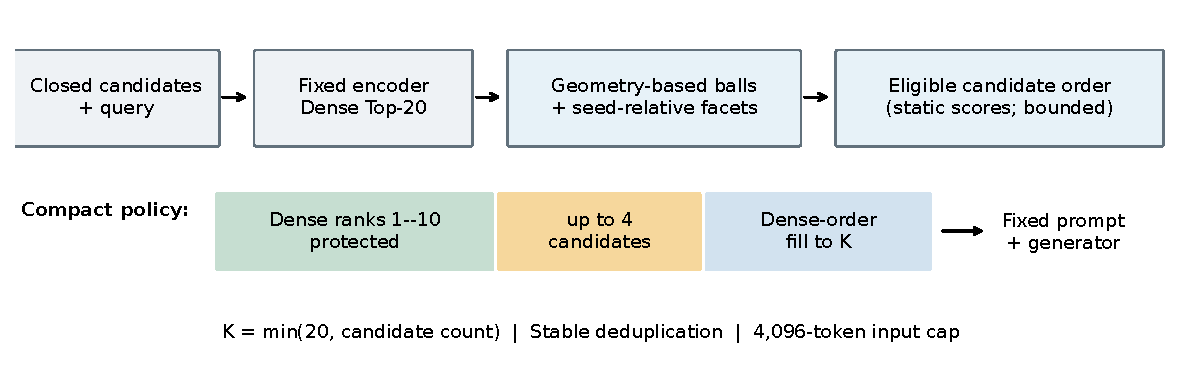
\includegraphics[width=.98\textwidth]{../shared/workflow.pdf}
\caption{The historical compact pipeline. Candidate groups cover the full
closed candidate set. Selection is static relative to the seeds; the protected
prefix, candidate placement, dense-order fill, and subsequent token cap are
separate operations. No answer label enters retrieval or prompting.}
\label{fig:workflow}
\end{figure*}

\subsection{Two Extensions around BGE}
The cross-space \emph{sidecar} keeps BGE's primary ranking and uses the frozen
MiniLM structure to propose candidates outside BGE Top-20. Its protected and
unprotected arms use the same insertion candidates but place them after the
prefix or at the front, respectively.

The \emph{native} variant reconstructs groups and relative scores in BGE
space. Development selected one of 16 configurations, with leaf target six,
four insertion slots, unit-score percentile floor $.50$, and broad relative
facet gates. The split depth, balance gate, score normalization, and candidate
score differ from the compact method (Appendix~\ref{app:native}).
This is a related implementation, not an encoder-only substitution.
None of the results below comes from the later dynamic-selection prototypes.

\section{Experimental Design}
\subsection{Questions and Comparisons}
We use HotpotQA training distractor candidates and the answerable MuSiQue
training candidate sets \citep{yang2018hotpotqa,trivedi2022musique}.
The compact evaluations contain 1,000 HotpotQA questions, 3,000 MuSiQue
questions, and a separate joint component set of 1,000 and 1,500 questions.
The sidecar and native confirmation studies each use another 1,000/1,500
set. Their frozen identity manifests record exclusion of the preceding
evaluation boundaries. These are project-held-out subsets of training
releases, not official hidden test submissions.

The joint component study includes MiniLM Dense, BM25, a Dense--BM25 hybrid,
BGE large-en-v1.5, \full, NoFacet, and NoProtection.
NoFacet retains compact ball geometry but uses centroid-only expansion.
NoProtection changes the placement policy. Neither is a flat-unit or
budget-matched MMR control.
Native development uses 500 HotpotQA and 750 MuSiQue questions, separate from
confirmation. Its small positive development difference selects a
configuration; it is not pooled with confirmation.

\subsection{Generation and Metrics}
The principal generator is Qwen2.5-1.5B-Instruct FP16 on an RTX 4060 Laptop
8GB. A fixed short-answer prompt requests an answer from the evidence or
\texttt{UNKNOWN}. Generation is greedy, batch size one, with at most 32 new
tokens and a 4,096-token input cap. A transfer study uses the same initial
rankings with Gemma 4 E2B in the official mobile-QAT deployment format.
That comparison concerns these deployment configurations, not pure model
architecture or device-independent efficiency.

We report mean answer F1 and exact match (EM). Complete recall (CR@20)
records whether all annotated supporting evidence is covered; evidence recall
(ER@20) records the covered fraction. HotpotQA has sentence-level support
labels, whereas MuSiQue uses supporting paragraphs. MuSiQue coverage therefore
must not be described as sentence-chain recall.

The initial HotpotQA and generator-transfer scorers include the special-answer
F1 rule for yes/no/noanswer; the MuSiQue scorer uses answer aliases.
The joint component, sidecar, and native studies use their frozen
alias-max normalized token-overlap implementation without HotpotQA's
special-answer exception. We label these \emph{legacy scoring} results and
retain them unchanged. The impact on actual predictions has not been
quantified, so these rows are not asserted to reproduce official HotpotQA
leaderboard metrics.

\subsection{Estimates and Uncertainty}
For paired per-query scores, the target is the mean within-query difference.
Joint studies average the two dataset means with equal weight. Their 10,000
bootstrap draws resample queries within each dataset, preserving method
pairing; we reproduce the recorded percentile intervals rather than
re-estimating them. The intervals describe the frozen query-sampling model,
not uncertainty over model training or alternative development searches.

Statistical tests require a null distribution and suitable sampling assumptions
\citep{dror2018hitchhiker}. Some historical decision files call an uncentered
bootstrap nonpositive-tail fraction a one-sided p-value and apply Holm
adjustment. Its general null calibration was not established. We preserve the
recorded decisions for provenance, but base the present description on effect
estimates and intervals, without claiming a newly validated familywise test.
Intervals crossing zero are unresolved, not equivalent. Shared source
documents can induce dependencies not captured by query-level resampling.

\section{Results}
\subsection{Does Completion Help Compact Retrieval?}
Yes, within the tested compact configuration. Table~\ref{tab:compact} shows
positive effects on the initial HotpotQA and MuSiQue sets and the separate
component set. Their recorded 95\% intervals exclude zero, with absolute
F1 differences between $.01140$ and $.01478$. The initial HotpotQA lower
bound is close to zero, so the magnitude and uncertainty are more informative
than a binary success label.

\begin{table*}[t]
\centering\small
\begin{tabular}{@{}lccccc@{}}
\toprule
Evaluation set & Queries & Dense F1 & Full F1 & $\Delta$F1 & 95\% interval\\
\midrule
HotpotQA & 1,000 & .42150 & .43628 & $\effHotpot$ & $\ciHotpot$\\
MuSiQue & 3,000 & .13595 & .14735 & $\effMusique$ & $\ciMusique$\\
Joint component$^\dagger$ & 2,500 & .30446 & .31803 & $\effJoint$ & $\ciJoint$\\
\bottomrule
\end{tabular}
\caption{Compact MiniLM with Qwen. Scores are on the 0--1 scale. The joint row
is dataset-equal-weighted, not a pooled average of all 2,500 questions.
$^\dagger$Legacy scoring as defined in Section~4.2. All numbers reuse
the frozen results.}
\label{tab:compact}
\end{table*}

Retrieval coverage also increases: CR@20 rises from $.737$ to $.798$ on
HotpotQA and from $.589$ to $.650$ on MuSiQue. These are different support
granularities, and neither change by itself measures answer improvement.
The corresponding answer gains supply the end-to-end evidence.

\subsection{What Do the Component Contrasts Identify?}
On the joint compact set, \full minus NoFacet is $\effFacet$
with interval $\ciFacet$. This favors the particular facet-conditioned
selector over centroid-only expansion. It does not show that hyperedges are
necessary, or that higher-order structure explains more than a simpler
coverage heuristic. \full minus NoProtection is $\effProtection$
$\ciProtection$, leaving the independent benefit of protection unresolved
in that compact setting.

In the sidecar study, Protected minus Unprotected is $\effSidecarPlace$
$\ciSidecarPlace$. Protected insertion is better than the tested front
insertion policy. Yet Protected minus BGE remains unresolved; avoiding part of
an intervention's damage is different from improving the untouched baseline.
The native facet and placement contrasts also cross zero
(Figure~\ref{fig:components}).

\subsection{Does the Benefit Extend to Strong Retrieval?}
The original compact \full is below BGE on the same component set:
$\effStrong$ $\ciStrong$. BM25 and the hybrid are additional comparators,
with \full differences of $\effBm$ $\ciBm$ and
$\effHybrid$ $\ciHybrid$, respectively.
Neither interval resolves a difference.

The two BGE extensions address more specific alternatives.
The sidecar adds candidates from the existing compact structure; its
Protected-minus-BGE effect is $\effSidecar$ $\ciSidecar$.
Rebuilding the geometry natively in BGE yields $\effNative$ $\ciNative$.
Both point estimates are slightly negative, and both intervals cross zero.
These findings do not establish complementarity with BGE, but they are not
equivalence tests. Because the configurations and query sets differ, the three
BGE comparisons are not a causal dose--response curve for retriever strength.

\begin{figure*}[t]
\centering
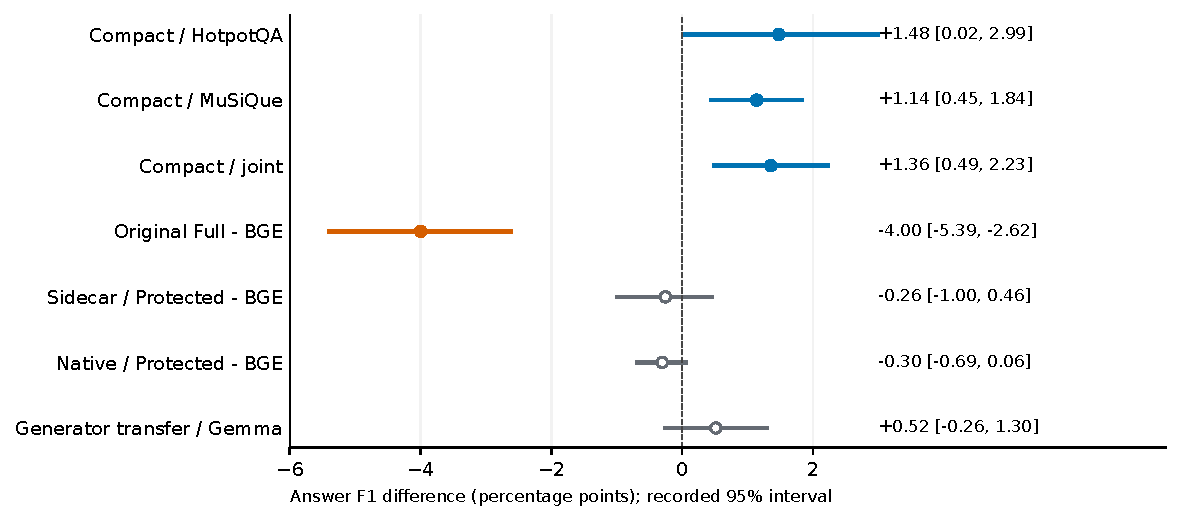
\includegraphics[width=.98\textwidth]{../shared/effects.pdf}
\caption{Paired answer-F1 effects in percentage points (one point is $.01$
on the score scale). Each interval is the recorded 95\% percentile bootstrap
interval for that row's comparison; rows are not pooled. Open markers denote
intervals crossing zero. Joint, original-versus-BGE, sidecar, and native rows
use legacy scoring.}
\label{fig:effects}
\end{figure*}

\subsection{Does the Result Transfer to Another Generator?}
With the fixed Gemma mobile-QAT configuration, the equal-weight
\full-minus-Dense effect is $\effGemma$ $\ciGemma$.
This result does not establish generator transfer. The rankings are reused
from the initial studies, so this is an intervention on the tested generator
deployment, not an additional independent retrieval sample. Differences in
format and runtime prevent interpretation as a controlled architecture
comparison between Qwen and Gemma.

\begin{figure*}[t]
\centering
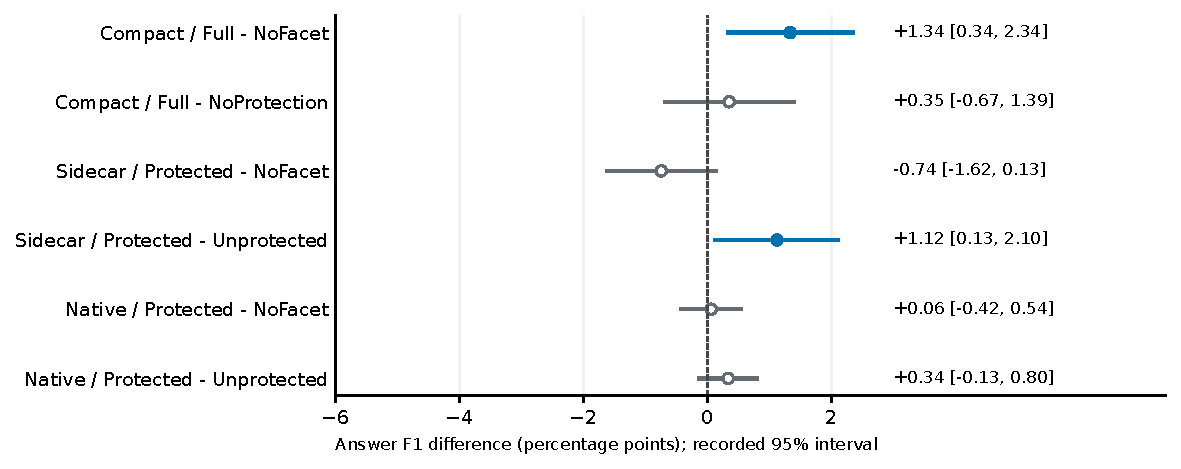
\includegraphics[width=.98\textwidth]{../shared/components.pdf}
\caption{Component contrasts under legacy scoring. NoFacet is a specific
historical comparator; native NoFacet also changes the candidate-score
coefficients, so that row is a pipeline contrast rather than a pure removal of
one coefficient. Placement comparisons retain insertion candidates but do not
establish identity of the actual truncated prompt evidence.}
\label{fig:components}
\end{figure*}

\section{Analysis and Implications}
\subsection{Adding Evidence Can Also Displace It}
The post-decision sidecar audit counts 21 added and 29 displaced annotated
supporting units in HotpotQA, and 59 added versus 50 displaced in MuSiQue.
The corresponding native counts are 3/2 and 16/15.
Thus, native completion has a net $+1$ supporting unit in each dataset while
both answer-F1 point estimates are negative. These totals concern annotated
evidence identities at each dataset's support granularity, not complete
reasoning chains or a causal effect per inserted unit.

A gain can fail to reach the answer because retained evidence is redundant,
an essential fact is displaced, or the generator fails to use the context.
The aggregate counts do not distinguish these mechanisms. They demonstrate
why selection, final ranking, prompt-visible evidence, and answer quality
should be measured separately.

\subsection{What Geometry Does and Does Not Establish}
For unit vectors $x_i$ in a ball, compactness is
\begin{equation}
C(B)=\frac{\|\sum_{i\in B}x_i\|}{|B|}.
\end{equation}
For any partition $B=\bigsqcup_j B_j$, the triangle inequality gives
\begin{equation}
\sum_j\frac{|B_j|}{|B|}C(B_j)\geq C(B).
\end{equation}
This holds for arbitrary partitions. An increase in weighted child
compactness therefore cannot alone validate a semantic split. The zero-sum
scalar extends continuously to zero, although its normalized center is
undefined without an implementation convention.
These facts clarify the historical representation; they neither invalidate
the observed compact gains nor independently explain them.

\subsection{Evidence for a Layer, Not an Indispensable Component}
The tested pipeline can improve a compact backbone without demonstrating that
every named component is necessary. Ordinary clusters, MMR, and sentence-level
coverage remain plausible alternatives. A decisive comparison would match
candidate access, intervention budget, group count, and generator context.
The absence of that comparison narrows the present contribution to a complete
pipeline and specific component contrasts.

Similarly, the cross-space placement result does not prove that moving
identical final evidence changes the answer. Final Top-20 membership and
token truncation must also be controlled for that claim. A protected policy
can help through preserving evidence, through order, or through both.

\section{Limitations}
All answer-quality results use closed benchmark candidate sets. They do not
measure corpus reachability, ANN recall, full-wiki indexing, or open-domain
noise. The positive compact evidence uses one retriever, one principal
generator, one short-answer prompt, and Top-20. The additional generator and
BGE extensions are unresolved rather than demonstrations of broad robustness.

The radius gate is inactive in the historical compact split rule, and the
facet selector does not dynamically recompute coverage. A corrected or
dynamic implementation is a different method and has no formal result in this
paper. The native NoFacet score changes multiple coefficients; its effect is
not a pure component ablation. No fair ordinary-clustering or generic
coverage comparison has been completed.

Legacy evaluator compatibility and historical tail-probability calibration
limit the strength of statistical claims. We have not rescored predictions or
replaced the frozen inferential procedure. Query-disjoint samples are not
necessarily independent at the document or pretraining level. Dataset
training releases may have appeared in generator pretraining. Post-decision
mechanism summaries and representative cases do not identify causal
mediation, and finite resource-based sample sizes are not a power guarantee.

\section{Conclusion}
Structured evidence completion improves the tested compact MiniLM pipeline on
three closed-candidate multi-hop QA evaluations. A facet-conditioned selector
also exceeds its specified compact centroid-only comparator. The original
system remains below BGE, while cross-space and native BGE extensions do not
establish an incremental answer-quality benefit. Protection helps relative to
front insertion in one sidecar setting, but does not make its candidates useful
relative to BGE. The resulting design lesson is to evaluate completion jointly
with its backbone and displacement policy, using answer quality rather than
structural coverage alone as the endpoint.

\section*{Ethical and Reproducibility Considerations}
This study uses existing benchmark releases and model artifacts; it introduces
no new participant study. Negative and unresolved results are retained.
Source code, configurations, derived predictions, and result manifests exist
in the research repository. Third-party datasets and weights remain subject
to their original terms. An anonymous distribution and author-approved
licensing statement are required before submission. AI-assisted coding,
analysis preparation, and writing were used; responsibility for the submitted
work remains with the human authors.

\bibliography{../shared/references}
\appendix
\section{Historical Implementation and Provenance}
\label{app:native}
The compact method uses \texttt{all-MiniLM-L6-v2}; the strong ranking uses
\texttt{BAAI/bge-large-en-v1.5}. Native C10 uses depth limit eight,
minimum child fraction $.20$, and compactness-gain threshold $10^{-10}$.
Its two seed balls are ranked by query-score percentile, density percentile,
then identity. Broad gates require query-score percentile at least $.35$ and
density percentile at least $.25$. Eligible non-seed balls must contribute a
seed-relative new facet; at most four balls supply candidates.
Only units outside BGE Top-20 with unit-score percentile at least $.50$ are
eligible. Candidate scoring is
\begin{equation}
\begin{split}
h_u^{\mathrm{native}}={}&.45p_u+.25p_{b(u)}+.15p_{\rho(u)}\\
&+.10p_{C(u)}+.05\min(n_{b(u)},3)/3 ,
\end{split}
\end{equation}
where the $p$ terms are within-query empirical percentiles of unit relevance,
ball relevance, density, and compactness. Native NoFacet replaces this by
$.50p_u+.30p_{b(u)}+.10p_{\rho(u)}+.10p_{C(u)}$ and removes the new-facet
eligibility requirement. The comparison therefore changes both gating and
weights.

The paper's scientific names map to the frozen repository records as follows:
initial HotpotQA/MuSiQue to Stage4E/4F, generator transfer to Stage4G,
joint components to Stage4H, cross-space sidecar to Stage4I, and native
confirmation to Stage5A. Aggregate summaries, implementation configurations,
and the manuscript evidence ledger provide the exact artifact paths.
The later Stage6 development outputs, engineering repairs, and synthetic v2
prototype are excluded from these empirical results.

\paragraph{Verification scope.}
Historical verification records are retained as records of their original
checks. This manuscript revision cross-checks the reported aggregate values
and plotting inputs; it does not rerun retrieval, generation, Gold evaluation,
or bootstrap. Agreement of files or schemas cannot establish independent
semantic correctness, and subsequent verifier repairs are not retroactive
certification of the old experiments.

\paragraph{Complexity and measured cost.}
With embeddings available, recursive two-seed assignment costs
$O(H|U_q|d)$, scoring and sorting cost
$O(|U_q|\log|U_q|+|{\cal B}_q|d+|{\cal B}_q|\log|{\cal B}_q|)$,
and working memory is $O(|U_q|d+|U_q|+|{\cal B}_q|)$, excluding tokenization
and model inference. The native confirmation records 8.544\,s retrieval
reconstruction, 887.650\,s BGE generation, 884.198\,s protected-native
generation, and 3.592\,GiB peak GPU memory. These are transaction-specific
measurements, not corpus-index costs or a controlled speed advantage.
\end{document}
